% See exam.cls and examdoc.tex for the license information
\documentclass[12pt, answers]{exam}

\usepackage{amssymb}
\usepackage{makeidx}
\usepackage{amsmath}
\usepackage{graphicx}
\usepackage{caption}
\usepackage{tabulary}
\usepackage{color}
\usepackage{multicol}
\usepackage{amsmath}
\usepackage{multirow}
\usepackage{enumerate}
\usepackage{float}

\usepackage{array}
\newcolumntype{C}[1]{>{\centering\let\newline\\\arraybackslash\hspace{0pt}}m{#1}}

\addpoints

% In case we're not using hyperref.sty:
\providecommand{\texorpdfstring}[2]{#1}
% The following can be used in \section commands
% without generating pdf warnings:
\newcommand{\bs}{\texorpdfstring{\char`\\}{}}

\makeindex

\newcommand{\indc}[1]{\index{#1@\texttt{\char`\\#1}}}
\newcommand{\indcsub}[2]{\index{#1@\texttt{\char`\\#1}!#2}}
\newcommand{\indcstart}[1]{\index{#1@\texttt{\char`\\#1}|(}}
\newcommand{\indcstop}[1]{\index{#1@\texttt{\char`\\#1}|)}}

\newcommand{\indt}[1]{\index{#1@\texttt{#1}}}
\newcommand{\indtsub}[2]{\index{#1@\texttt{#1}!#2}}
\newcommand{\indtstart}[1]{\index{#1@\texttt{#1}|(}}
\newcommand{\indtstop}[1]{\index{#1@\texttt{#1}|)}}

\extraheadheight{-.4in}

\pagestyle{headandfoot}
%\extraheadheight{.2 in}
\firstpageheader{}{}{}
\runningheader{}{}{}
\firstpagefooter{INF281}{Exercise 04}{Page \thepage\ of \numpages}
\firstpagefootrule
\runningfooter{INF281}{Exercise 04}{Page \thepage\ of \numpages}
\runningfootrule

%---------------------------------------------------------------------

\shadedsolutions
%\noprintanswers
\definecolor{SolutionColor}{rgb}{0.8,0.9,1}

\begin{document}

\section*{INF281 Exercise 04 solutions}

%---------------------------------------------------------------------
\begin{questions}

%%% Question 1
\question \textbf{Local alignment with DP}
  
The DP algorithm can be used to identify optimal local alignments. Assume the scoring scheme as match: 1, mismatch: -1, and gap penalty: 1.

\vspace{0.1 in}

\begin{parts}

%% (a)
  \part Complete the DP table to find the optimal local alignment.

\begin{figure}[h]
      \centering
      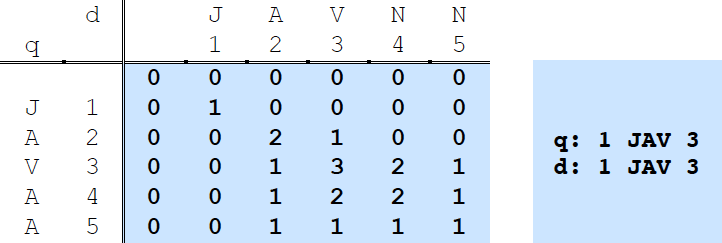
\includegraphics[width=0.7 \textwidth]{fig04/local_dp_solution.png}
\end{figure}

%% (b)
\part Backtrack from $H_{9,6}$ and write down the local alignment.  

\begin{figure}[h]
      \centering
      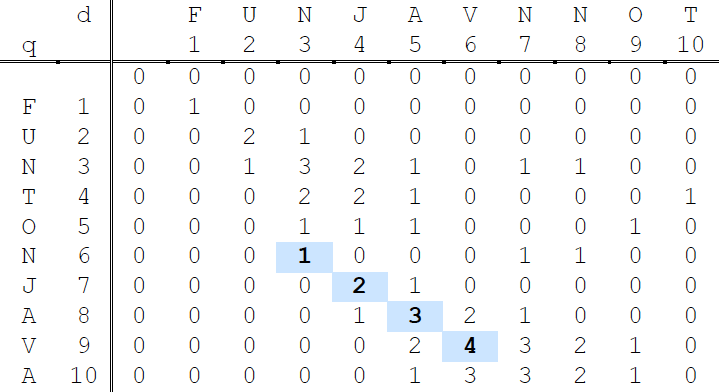
\includegraphics[width=0.75 \textwidth]{fig04/local_dp_backtrack_solution.png}
\end{figure}

\begin{solution}[0.75 in]
\begin{verbatim}
  q: 6 NJAV 9
  d: 3 NJAV 6
\end{verbatim}
\end{solution}

\end{parts}


\newpage

%%% Question 2
\question \textbf{Dot matrix}
  
A dot matrix is one of the simplest methods to identify local alignments. 

\vspace{0.1 in}

\begin{parts}

%% (a)
  \part Fill the table with dots.

\begin{figure}[h]
      \centering
      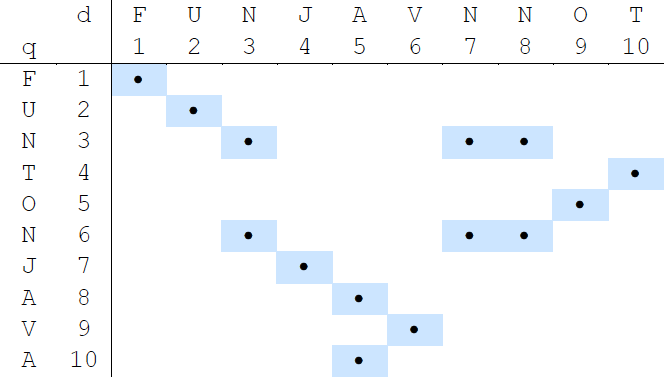
\includegraphics[width=0.7 \textwidth]{fig04/dot_matrix_solution.png}
\end{figure}

%% (b)
\part Identify all segment pairs with at least 3 contiguous dots along diagonals.

\begin{solution}[0.75 in]
\begin{verbatim}
  q: 1 FUN 3        q: 6 NJAV 9
  d: 1 FUN 3        d: 3 NJAV 6
\end{verbatim}
\end{solution}

%% (c)
\part Identify all segment pairs with at least 3 contiguous dots along aniti-diagonals.

\begin{solution}[0.75 in]
\begin{verbatim}
  q: 4 TON 6
  d: 8 NOT 10
\end{verbatim}
\end{solution}

\end{parts}



%%% Question 3
\question \textbf{N-grams}
  
N-grams are n-letter words that can be used for database search methods. Create a table of 2-grams for q: ATGCAT.

\vspace{0.1 in}

\begin{parts}

%% (a)
  \part List all 2-grams of q.

\begin{solution}[0.5 in]
\begin{verbatim}
  AT, TG, GC, CA, AT
\end{verbatim}
\end{solution}

%% (b)
\part Fill the table with the 2-grams and the corresponding indices of q.

\begin{figure}[H]
      \centering
      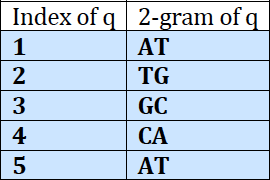
\includegraphics[width=0.25 \textwidth]{fig05/n-gram_solution.png}
\end{figure}

\end{parts}



%%% Question 4
\question \textbf{Matching n-grams}
  
Calculate the scores of the segment pairs between q: CG and all 2-gram permutations of \{A, C, G, T\}.

\medskip 

Score matrix:
\begin{figure}[H]
      \centering
      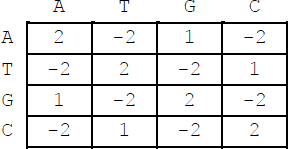
\includegraphics[width=0.25 \textwidth]{fig05/score_scheme_1.png}
\end{figure}

\vspace{0.1 in}

\begin{parts}

%% (a)
  \part Fill the scores between CG and all its matching n-grams.

\begin{figure}[H]
      \centering
      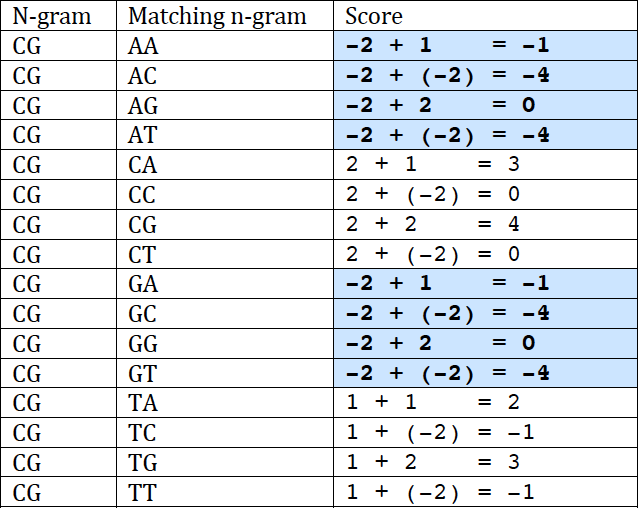
\includegraphics[width=0.6 \textwidth]{fig05/matching_n-gram_solution.png}
\end{figure}

%% (b)
\part Identify all matching n-grams when the threshold value T is 3.

\begin{solution}[0.5 in]
\begin{verbatim}
  CA, CG, TG
\end{verbatim}
\end{solution}

\end{parts}



%%% Question 5
\question \textbf{Lookup table for n-grams}
  
Create a 2-gram lookup table with indices and scores for the sequence q: ATGCAT. 

\medskip 

Score matrix:
\begin{figure}[H]
      \centering
      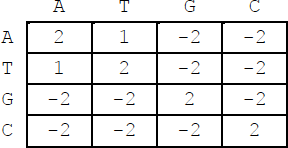
\includegraphics[width=0.25 \textwidth]{fig05/score_scheme_2.png}
\end{figure}

 T: 3 \\

Pre-calculated scores of all segment pairs:
\begin{figure}[H]
      \centering
      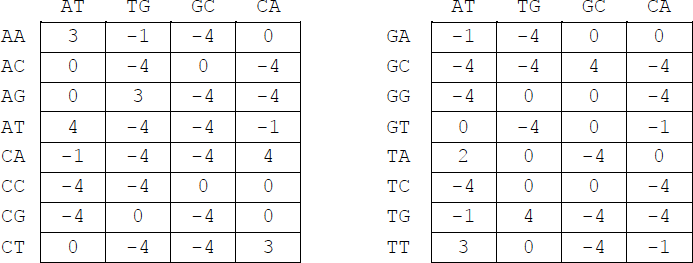
\includegraphics[width=0.65 \textwidth]{fig05/lookup_table_precalculated.png}
\end{figure}

\begin{parts}

%% (a)
  \part Fill the table.

\begin{figure}[H]
      \centering
      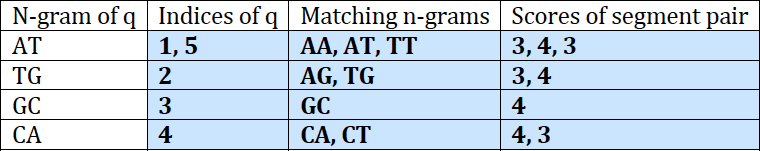
\includegraphics[width=0.65 \textwidth]{fig05/lookup_table_n-gram_solution.png}
\end{figure}

%% (b)
\part Create a lookup table for the matching n-grams with scores and indices.

\begin{figure}[H]
      \centering
      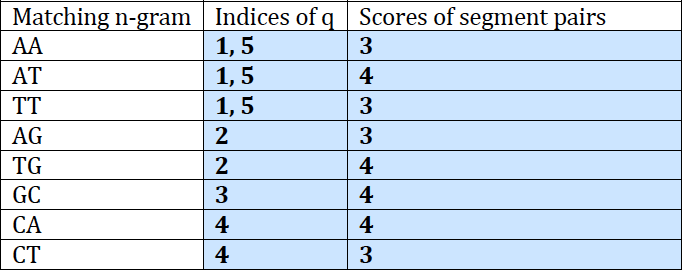
\includegraphics[width=0.6 \textwidth]{fig05/lookup_table_n-gram_final_solution.png}
\end{figure}

\end{parts}
\newpage

%%% Question 6
\question \textbf{Finite-state machine with 2-grams}
  
Use the 2-gram lookup table of q = ATGCAT to create a finite-state machine for all potential matching 2-grams.

\vspace{0.1 in}

Lookup table of 2-gram:
\begin{table}[h]
\centering
\begin{tabular}{|l|l|l|}
\hline
\textbf{Matching 2-gram} & \textbf{Indices of q} & \textbf{Scores of segment pairs} \\ \hline
AT                       & 1, 5                  & 4, 4                             \\ \hline
AA                       & 1, 5                  & 3, 3                             \\ \hline
TT                       & 1, 5                  & 3, 3                             \\ \hline
TG                       & 2                     & 4                                \\ \hline
AG                       & 2                     & 3                                \\ \hline
GC                       & 3                     & 4                                \\ \hline
CA                       & 4                     & 4                                \\ \hline
CT                       & 4                     & 3                                \\ \hline
\end{tabular}
\end{table}

\vspace{0.1 in}

\begin{parts}

%% (a)
  \part Add indices and scores to the corresponding edges. 

\begin{figure}[H]
      \centering
      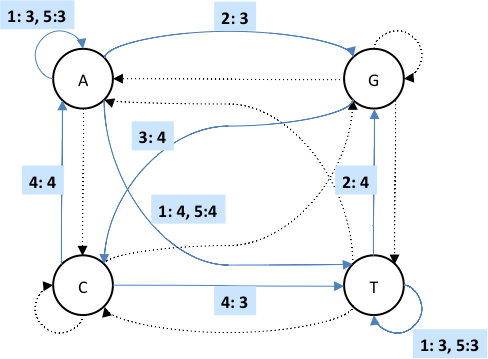
\includegraphics[width=0.45 \textwidth]{fig05/fsm_solution.png}
\end{figure}

%% (b)
\part Use the finite-state machine to find the matching segment pairs and the scores.

\begin{enumerate}
\item d1: TCGGTAA

\begin{solution}[0.5 in]
\begin{verbatim}
q: 1 AT 2    Score: 3    q: 5 AT 6    Score: 3
d: 6 AA 7                d: 6 AA 7
\end{verbatim}
\end{solution}

\item d2: ATAGC

\begin{solution}[1 in]
\begin{verbatim}
q: 1 AT 2    Score: 4    q: 5 AT 6    Score: 4
d: 1 AT 2                d: 1 AT 2

q: 2 TG 3    Score: 3    q: 3 GC 4    Score: 4
d: 3 AG 4                d: 4 GC 5
\end{verbatim}
\end{solution}

\end{enumerate}

\end{parts}


\newpage

%%% Question 7
\question \textbf{Finite-state machine with 3-grams}
  
Add edges to connect nodes to create an overlap graph that can be used as a 3-gram finite-state machine.

\vspace{0.1 in}

\begin{parts}

%% (a)
  \part List all 3-grams of AAACGGTA.

\begin{solution}[0.5 in]
\begin{verbatim}
AAA, AAC, ACG, CGG, GGT, GTA
\end{verbatim}
\end{solution}

%% (b)
\part Add edges that correspond to the 3-grams of AAACGGTA.

\begin{figure}[H]
      \centering
      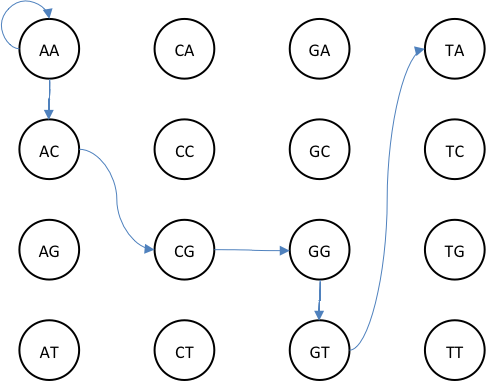
\includegraphics[width=0.45 \textwidth]{fig05/fsm2_solution.png}
\end{figure}

\end{parts}




\end{questions}
%---------------------------------------------------------------------
       
\end{document}

